\documentclass[conference]{IEEEtran}
\IEEEoverridecommandlockouts
% The preceding line is only needed to identify funding in the first footnote. If that is unneeded, please comment it out.
\usepackage{cite}
\usepackage{amsmath,amssymb,amsfonts}
\usepackage{algorithmic}
\usepackage{graphicx}
\usepackage{textcomp}
\usepackage{xcolor}
\def\BibTeX{{\rm B\kern-.05em{\sc i\kern-.025em b}\kern-.08em
    T\kern-.1667em\lower.7ex\hbox{E}\kern-.125emX}}
\begin{document}

\title{Natural Language Question Answer Pair Generation\\
}

\author{\IEEEauthorblockN{Satwik Muthyam}
\IEEEauthorblockA{\textit{16IT119} \\
\textit{Information Technology}\\
\textit{muthyamsatwik@gmail.com} 
}
\and
\IEEEauthorblockN{Sai Manikanta Badugu}
\IEEEauthorblockA{\textit{16IT209} \\
\textit{Information Technology}\\
\textit{saimanikanta189@gmail.com}
}
}

\maketitle

\begin{abstract}
Knowledge graphs such as Freebase that capture facts regarding entities and relationships between them have been used actively for responsive factoid questions. In this project, we have a tendency to explore the problem of mechanically generating question answer pairs from a given knowledge graph. The generated question answer (QA) pairs are often employed in many downstream applications. The generated QA pairs could be used for coaching higher QA systems. To come up with such QA pairs, we first extract a collection of keywords from entities and relationships expressed in a  triple stored within the knowlegde graph. From each such set, we plan to use a set of keywords to generate a language question that has a unique answer. We then propose a sequence to sequence model RNN to form question answer pairs from the previously taken keyword tuples from the knowledge graph. Our model generates QA pairs with a BLEU score of 58.2.

\end{abstract}


\section{Introduction}
The Knowledge Graph is a widely used data form by Google to improve the effectiveness of the search results  by providing data collected from different sources .This information is shown to users in an info box next to the search results. 

From the knowledge graph we extract the information in the form of triples. We classify each
node in the graph as either subject or object and the egde between the nodes the
relation(predicate).

We take a triple having of a subject, predicate and object. Subject is defined over a domain
while the object is defined over a range. The predicate gives the relationship between the
subject and the range and each predicate mayhave multiple subject object pairs associated
with it. In this model we consider only the case where the predicate is linked to a unique
subject and object pair.

The keyword triples generated is used as a input to the model for Question generation and to give out a unique answer. For this, it is important to first select a subset of triples from which interesting and meaningful questions can be constructed. Further, even for an interesting triple, it may be possible to use only certain subsets of keywords to construct a meaningful question. We need to automatically identify the right set of keywords that should be used to form the question such that the answer also lies in the set. In this project we not only generate QA pairs but also propose a model to extract important keywords in the form of tuples from the knowledge graph given.
\newline

An example set of keywords constructed
from the triple Capital(India, New Delhi)

Q: What is the capital of India?

A: New Delhi

Q: In which country is New Delhi?

A: India

We propose an RNN model which is trained over a set of questions taken from Wikianswers which consists of av variety of topics in it. We then used the keyword tuples generated in the previous step as input to the RNN model to generate a question with a unique answer associated with it.

\section{Literature Survey}
A number of papers have checked out the matter of generating vocabulary queries like WordNet(1990) and spacing similarity techniques. There are various works in automatic question generation from text. Many
proposed ways based on syntax based ways that use the grammatic structure of sentences, determine key
phrases and apply some transformation rules to make queries. Mannem et al. (2010) further used labeling for transformation rules. Cai et al. (2006) proposed associate XML nomenclature that used to manually produce question templates. This is sensitive to the performance of syntactical and linguistics parsing. Heilman and Smith (2010) used a rule based approach to remodel a declarative sentence into many candidate queries and rank them employing a supplying regression model. These approaches involve making templates manually
and so need vast manual work and have low recall. 

A problem that has been studied recently and is similar to our drawback of generating queries using data graph is that of generating queries from net queries. The motivation here is to mechanically generate queries from queries for community-based question respondent services such as WikiAnswers. The idea was implemmented by Lin and more developed by Zhao and Zheng. Each of those approaches were guide based approaches where the templates were made to learn using a vast question corpus along side question logs. Dror et al. (2013) planned a learning to rank based technique to get grammatically correct and various queries from a given question where the candidate queries were measured by the model proposed by Zhao. These approaches use several question pairs to find out question templates and so have higher generalization performance compared to earlier methods wherever templates were learnt manually.

The most recent work is done by Seyler et al. (2015) who proposed a method to come up with language queries
from data graphs given a subject of interest. They conjointly offer a technique to estimate problem
of generated queries. The generation of question is done by manually created patterns and therefore is prescribed in application. In distinction we propose associate RNN based mostly technique to find out
generation of language queries from a set of keywords. The model is trained using a dataset containing open domain keywords and question pairs.

\section{Motivation}
Knowledge graph is a data structure that increasingly came into use to store data and extract information. Also generating natural language questions from keywords is a difficult task. This motivates us to generate question answer pairs from knowledge graph using deep learning model. The generated question answer pairs can be used in several applications like training better QA systems.

Generation of questions from a given data has always been an issue because of the syntax and semantics involved in the  grammar. Many template based and syntax based models were proposed. But these models proved to be tidious and time consuming. So we came up with a deep learning which takes into account, the syntax and perform better in terms of speed and accuracy.
\section{Problem Statement}
Generation of Natural langauge question answer pairs from a given knowledge graph using a RNN model.
\section{Objectives}
\begin{itemize}
\item To extract information from a given knowledge graph. The data in the knowledge graph is present in the graph as nodes and edges connecting them. Information is taken from it by forming triples using the edges in the graph.
\item To generate natural language question answer pairs which are unique. Each question generated is topic specific and the set of keywords used in it are taken from a knowledge graph.

\item To train a RNN model which gives reliable questions to further develop a query system. The RNN model generates questions by taking the keywords generated from the knowledge graph. It is trained a dataset from Wikianswers.
\end{itemize}

\section{Proposed Work}
Let KG be the information graph that contains information regarding numerous entities within the variety of
triples. A triple consists of an subject, a predicate and associated object. Subjects and objects are present in the form of nodes in the KG, that might represent someone, a place, an abstract conception or a physical entity. Predicates are edges within the KG. They outline kind of relationship between the topic and the object. The framework to get QA pairs consists two major modules. the primary module, Question
Keywords and Answer Extractor, is language independent and extracts needed information about the entity E from the KG. The second module may be a language dependent RNN, primarily based Natural Language Question Generator. When fed with the knowledge extracted from the primary half it generates language QA pairs.

In order to retrieve data concerning the given entity E, we want to initially determine the node n that
represents the entity E within the KG. One way to identify node n is to leverage the label property.
The next step is to retrieve all the neighbours of n. Let m be a neighbour of n in KG, connected
by a predicate p. 

\begin{figure}[htpb]
\centerline{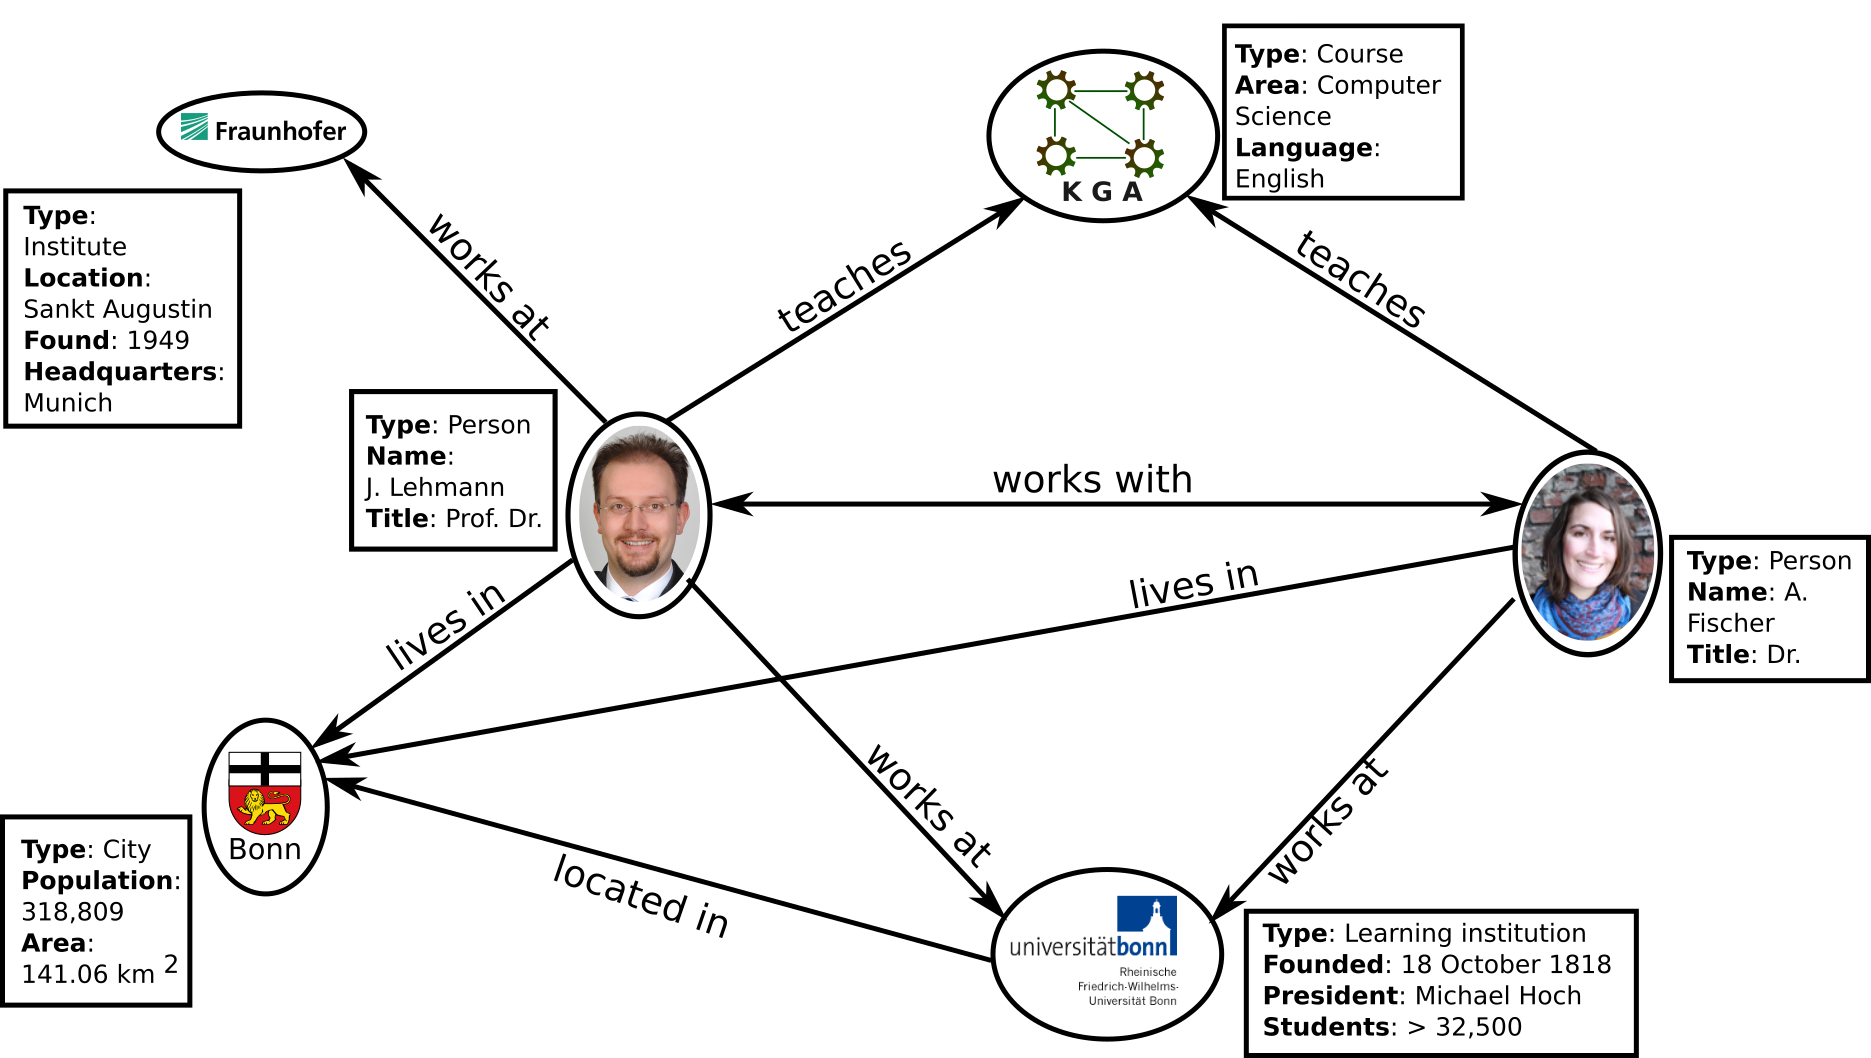
\includegraphics[height=7cm,width=8cm]{kg.png}}
\caption{Entity London in the Knowledge Graph}
\label{fig}
\end{figure}
Figure 1 shows the knowledge graph with 6 entities each connected to their respective objects through the predicates. For instance J.Lehmann is connected to Bonn through the predicate 'lives in'.Each of those neighbours are connected to the entity by a predicate. Given a predicate p, let sub(p) be the subject of p and obj(p) be the object of p. A predicate is usually outlined with a domain (subject type) and a range (object type) to produce higher linguistics. The domain and range defines the entity sorts that can be used because the subject and object of the predicate respectively. Let domain(p) and range(p) be the domain and range of p. Let {sub(p),dom(p),p,obj(p),range(p)} be the 5-tuple related to each p. 

We then describe QKA pairs are produced from 5-tuple. Let Qk be the question keywords set and Ak be the solution to the question to be generated using Qk. (Qk, Ak) along can kind a QKA pair. 
\newline
\begin{figure*}[t]
\centerline{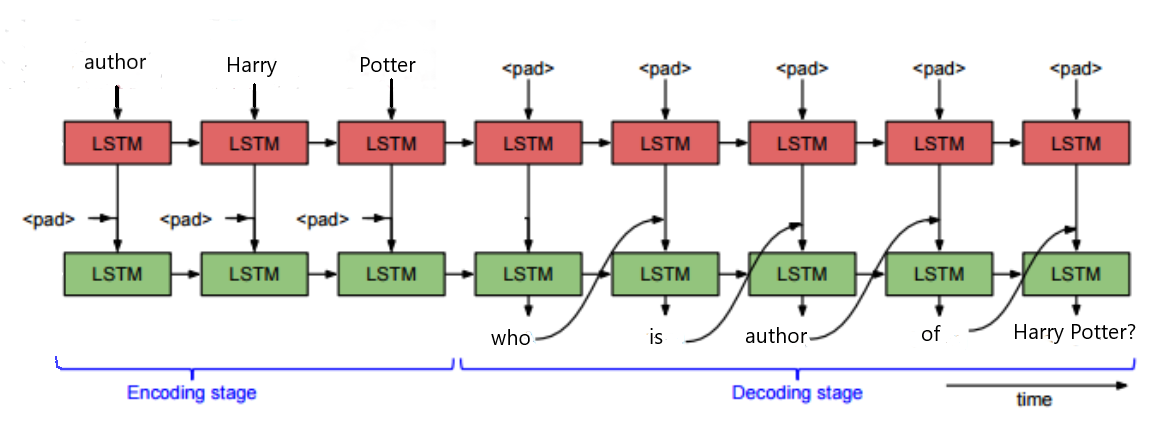
\includegraphics[height=8cm]{architecture.PNG}}
\caption{RNN architecture}
\label{fig}
\end{figure*}
\subsection{Unique Forward Relation}
If p is unique for sub(p) in KG, then Q can include sub(p), p and range(p). AK will be obj(p). If p is not unique for sub(p), then there may be multiple potential answers to the generated question as well as obj(p), and therefore we don't generate such a QK pair. For the instance of keyword pair {India, city}, we cannot generate a unique question answer pair since India has many instances of city.
\newline

\subsection{Unique Reverse Relation}
If p is unique for obj(p) in KG, then Q can include obj(p), p and domain(p). For example {Obama,President,USA} can generate a unique QA pair when the reverse relation is applied.
\newline

In the previous section, we put forward the approach for making question keywords and answer pairs. Then we proceed to model for generating natural language queries from a given set of question keywords. We make use of the keywords, QK = {qk1,qk2,.....,qkm}, as an input sequence and the question, Q = {q1,q2,....,qm}, as the output sequence. This style of treating a collection of keywords as a sequence and not as a bag of words allows us to come up with totally different semantically valid questions from a similar set K. For instance, given the question keywords, QK = {CEO, Google}, we can generate 2 semantically valid queries by changing the order of these words: (i) Who is the CEO of Google? and (ii) Does Google have a CEO?
We propose a Natural Language Question Generation (NLQG) model that initially encodes the input sequence using some distributed representation and then decodes the output sequence from this encoded sequence. Specifically, we use a RNN based encoder and decoder for language process tasks. 

Let m be the length of input sequencea we convert each word into vector of fixed size such that it's size is less than n. The encoder maps each seaquence of xi to a fixed size encoding. We use RNN model to find value of hi using the formula:
        hi = Φ(hi−1, xi)
where, hi ∈ <n is the hidden representation at position i. 
We make use of LSTM units as Φ for the implementation of our model. The decoder calculates the probability of the output from the encoded vector. The length of the output sequence may or may not be the same as that of the input sequence. 
The output sequence is divided into conditional probabilities and the the sequence with the highest probability is given as the question for the data provided.
\centerline{p(qj |q<j , hm) = t(qj−1, gj , hm)} 
where t is a non-linear function, that gives the probability of qj and gj is the decoder's hidden state.
\begin{table*}[t]

\begin{tabular}{|l|c|r|}
	\hline
	Keywords & Expected Sentences & Predicted Sentences\\
	\hline
    plays jacob black twilight movies & who plays jacob black in the twilight movies & what plays in twilight movies\\
	\hline
    see outside paris & what to see outside of paris & where is outside of paris\\
    \hline
    christopher play batman returns & who does christopher walken play in abtman returns & who is batman returns\\
    \hline
    contribution maurice wilkins make dna & what contribution did maurice wilkins make to dna & what is the contribution of maurice wilkins\\
    
	\hline
\end{tabular}
\end{table*}
To train the RNN model we make use of the keywords generated from the open domain CQA website. During the runtime the keywords generated are fed to the RNN model which gives a permutation of possible questions and the one highest probability is choosen from them.

\section{Experiments and Results}
\subsection{Dataset}
For training the K2Q-RNN model we need a set of keywords and question pairs. We use a large collection of open-domain queries taken from WikiAnswers. This dataset has around 20M queries. we have randomly chosen
1M queries from this corpus for coaching and 5k queries for testing (the most length of a question was restricted to fifty words). We extract keywords from the chosen queries by taking only Nouns, Verbs and Adjectives within the question. The components of speech tags were known using NLTK parts of speech package. We used the same order of the keywords taken from the question to maintain the meaning of the question.This sequence of keywords along side the initial question forms the input-output sequence used for
training.


\subsection{Results}
The experiments conducted yielded results with a better performance than the existing models. We used BLEU score to evaluate the RNN model. The model gave results with a BLEU score of 58.2 . The loss while building the model was less than 3.0. The predicted results and the actual results are shown in the figure 2. Column 1 shows the keywords used in the training of the RNN model. Column 2 shows the actual questions and column 3 shows the questions obtained from the RNN model.

The results of the QA pair generator is shown in fig 3. Column 1 shows the keywords fed to the RNN model. These keywords are taken from the knowledge graph in the form of triples and then converted into QKA pairs.
The second column shows the question generated for the given keywords and the next column shows the answer for the generated question. Each question generated in the model has a unique combination of Question and Answer.
\section{Conclusion}
In this project we proposed a way of generating QA pairs for a given entity employing a knowlwedge graph.
We also worked on generating QA pairs using RNN model trained with a dataset of varied questions. This model worked well giving better results than the manual generation and template based question generation which is tidious process. We have done evaluation for the model which showed that the model worked well.
This model can furthur be improved by adding features like stopword removal and addition of adverbs.

\section{Timeline of project}
\begin{figure}[htpb]
\centerline{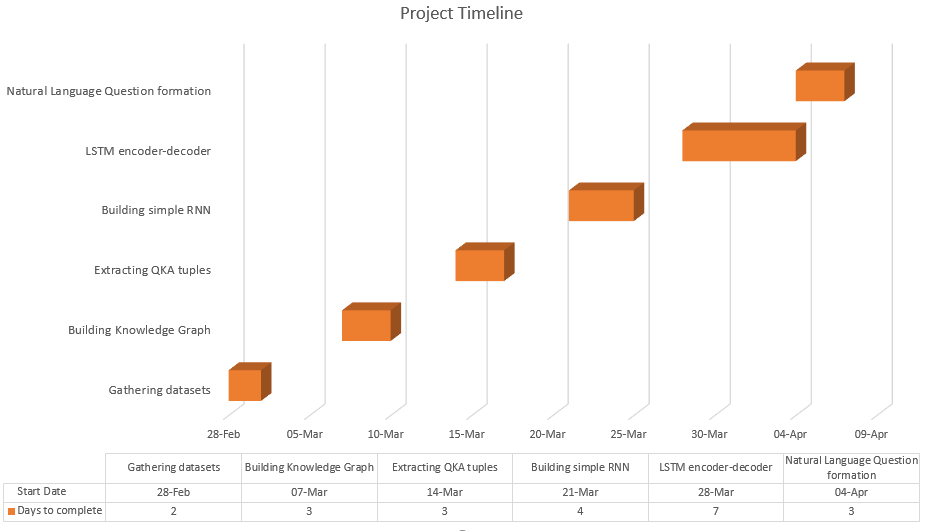
\includegraphics[height=8cm,width=8cm]{GanttChart.PNG}}
\caption{Timeline of the project}
\label{fig}
\end{figure}

\section{Individual Contribution}
\textbf{16IT119} – RNN Encoder/Decoder, KG Module Building, Word
Embeddings, Integration of modules

\textbf{16IT209} – Data Preprocessing QA Pair Generation,Simple RNN
model

\begin{thebibliography}{00}
\bibitem{b1} Sathish Indurthi, Dinesh Raghu, Mitesh M. Khapra and Sachindra Joshi "Generating Natural Language Question-Answer Pairs from a Knowledge Graph Using a RNN Based Question Generation Mode",Association for Computational Linguistics, 2017.

\bibitem{b2} Weiguo Zheng1, Jeffrey Xu Yu1, Lei Zou2, Hong Cheng, "Question Answering Over Knowledge Graphs: Question Understanding Via Template Decomposition",2018.
\end{thebibliography}
\begin{table}[]

\begin{tabular}{|l|c|r|}
	\hline
	Keywords & Predicted Sentences & Answer Extractor\\
	\hline
    Cuba treaties China & What are the treaties of Cuba & China\\
	\hline
    Bird exhibits behaviour & What bird exhibits in the? & Activities-Behaviour\\
    \hline
    China protests Countries & Who protests China? & India\\
    
	\hline
\end{tabular}
\end{table}

\end{document}

